
\documentclass[crop,tikz]{standalone}
\usepackage[utf8]{inputenc}
\usepackage{tikz}
\usepackage{pgfplots}
\pgfplotsset{compat=newest}
\usepgfplotslibrary{groupplots}
\begin{document}

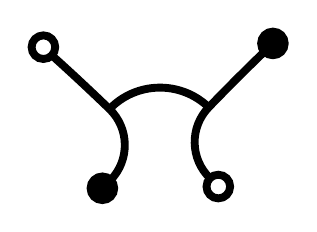
\begin{tikzpicture}[scale=1]
\def\col{black}
\def\lw{1mm}
\def\alpi{2.000000}
\def\beti{90.000000}
\def\gam{90.000000}
\def\alpii{2.000000}
\def\betii{90.000000}
\def\gamh{45.000000}

\def\eps{0.000000}
\def\ci{314.000000}
\def\cii{45.000000}
\def\ciii{226.000000}
\def\civ{135.000000}

\def\ri{28.647890}
\def\rii{0.636620}
\def\rg{0.891268}
\def\riii{28.647890}
\def\riv{0.636620}

\path (0.000000, 0.000000)coordinate(F1);

\draw[\col, line width=\lw] (F1)arc(180+\ci:180+\ci+\alpi:\ri)coordinate(OM);
\draw[\col, line width=\lw] (OM)arc(180+\ci+\alpi:180+\ci+\alpi+\beti:\rii)coordinate(F2);
\draw[\col, line width=\lw] (OM)arc(90+\ci+\alpi:90+\ci+\alpi+\gam:\rg)coordinate(UM);
\draw[\col, line width=\lw] (UM)arc(\gam+\ci+\alpi:\gam+\ci+\alpi+\alpii:\riii)coordinate(F3);
\draw[\col, line width=\lw] (UM)arc(\gam+\ci+\alpi:\gam+\ci+\alpi-\betii:\riv)coordinate(F4);

\draw[line width=\lw, fill=\col] (F1)++(404.000000 :.15) circle(.15);
\draw[line width=\lw] (F2)++(-45.000000 :.15) circle(.15);
\draw[line width=\lw] (F3)++(136.000000 :.15) circle(.15);
\draw[line width=\lw, fill=\col] (F4)++(225.000000 :.15) circle(.15);
% This file was created by matplotlib2tikz v0.6.18.

\end{tikzpicture}
%% End matplotlib2tikz content %% 
\end{document}